\section{} % Question 1
Given an HMM with the following properties:
$$
q=
	\begin{pmatrix}
		0.75 \\
		0.25
	\end{pmatrix}
	;
A=
	\begin{pmatrix}
		0.99 &  0.01 \\
		0.03 & 0.97
	\end{pmatrix}
	;
B=
	\begin{pmatrix}
		b_1(x) \\
		b_2(x)
	\end{pmatrix}
$$

To find the state probabilities at time $t+1$, we determine the state probabilities at $t$, in combination with the transition probabilities, as:

$$
P[S_{t+1}=j] 
	= \sum_{i=1}^{N} P[S_{t+1} = j \land S_t = i]
	= \sum_{i=1}^{N} a_{i j} P[S_t = i]
$$

As $t=2$:
$$P[S_2 = 1] = (0.99 \times 0.75) + (0.03 \times 0.25) = 0.75$$
$$P[S_2 = 2] = (0.01 \times 0.75) + (0.97 \times 0.25) = 0.25$$

Similarly, at $t=3$:
$$P[S_3 = 1] = (0.99 \times 0.75) + (0.03 \times 0.25) = 0.75$$
$$P[S_3 = 2] = (0.01 \times 0.75) + (0.97 \times 0.25) = 0.25$$

And so on for $S_t$ with higher values of $t$. Hence, $P[S_t = j]$ is constant for all $t$.

\section{} % Question 2
We tested this with the following MatLab code:

\begin{minted}[mathescape, linenos, numbersep=5pt, frame=lines, framesep=2mm, tabsize=4, numberblanklines=true, breaklines=true]{matlab}
num=10000;

%Generate ones and twos
mc2=MarkovChain([0.75;0.25], [0.99 0.01;0.03 0.97]);
onesTwos=rand(mc2, num);
percentageTwos=(sum(onesTwos)-num)/num*100;
disp(['percentage of ones: ', num2str(100-percentageTwos), '%']);
disp(['percentage of twos: ', num2str(percentageTwos), '%']);
\end{minted}

Which gives the following output:

\begin{minted}[mathescape, linenos, numbersep=5pt, frame=lines, framesep=2mm, tabsize=4, numberblanklines=true, breaklines=true]{matlab}
>> test
percentage of ones: 73.41%
percentage of twos: 26.59%
\end{minted}

The relative frequency of occurrences of $S_t = 1$ and $S_t = 2$ are 0.734 and 0.266 respectively. Thus, they are approximately equal to the theoretically calculated values.

%Skip question id 3, since it has no answer
%\setcounter{section}{3}

\section{} % Question 3
The expected value can be calculated by taking the weighted average of the expected values of the individual states:
\begin{align*}
E(X)
	&= E(X | S_{t-1} = 1) P(S_{t-1} = 1) + E(X | S_{t-1} = 2) P(S_{t-1} = 2)\\
	&= \mu_1 \times P(S_{t-1} = 1) + \mu_2 \times P(S_{t-1} = 2) \\
	&= 0 \times 0.75 + 3 \times 0.25
	&= 0.75
\end{align*}

The variance requires a bit more logic:
\begin{align*}
var(X)
	&= E_Z (var_X (X|Z)) + var_Z (E_X (X|Z))\\
	&= \left( \sum_{i=1}^{N} var(X_i) \times P(S_{t-1} = i) \right)
	 + \left( \sum_{i=1}^{N} E(var(X_i) \times P(S_{t-1} = i)\right)\\
	&= \left( \sigma_1^2 \times P(S_{t-1} =1) + \sigma_2^2 \times P(S_{t-1} =2)\right)
	 +  \left((\mu_1 - \mu_x)^2 \times P(S_{t-1} = 1) + (\mu_2 - \mu_x)^2 \times P(S_{t-1} = 2)\right)\\
	& = 1^2\times0.75 + 2^2\times0.25 + (0 - 0.75)^2 \times 0.75 + (3 - 0.75)^2 \times 0.25\\
	&= 3.4375
\end{align*}

We tested this with the following code:
\begin{minted}[mathescape, linenos, numbersep=5pt, frame=lines, framesep=2mm, tabsize=4, numberblanklines=true, breaklines=true]{matlab}
mc=MarkovChain([0.75;0.25], [0.99 0.01;0.03 0.97]);
g1=GaussD('Mean',0,'StDev',1); %distr for state 1
g2=GaussD('Mean',3,'StDev',2); %distr for state 2
h=HMM(mc, [g1; g2]);
x=rand(h, 5000);
%Get statistics about the numbers
disp(['mean:     ', num2str(mean(x))]);
disp(['variance: ', num2str(var(x))]);

>> mean: 0.67065
>> variance: 3.2403
\end{minted}

\section{} % Question 4
As shown in figure~\ref{fig:question_4_HMM_plot}, though the output of the HMM is random, it still follows the probability distribution of the states 1 and 2, i.e. almost 75\% of the HMM output is at state 1 and 25\% of them are at state 2.

\begin{figure}[H]
	\caption{HMM output plot with $N(0,1)$ and $N(3,2)$}
	\label{fig:question_4_HMM_plot}
	\centering
	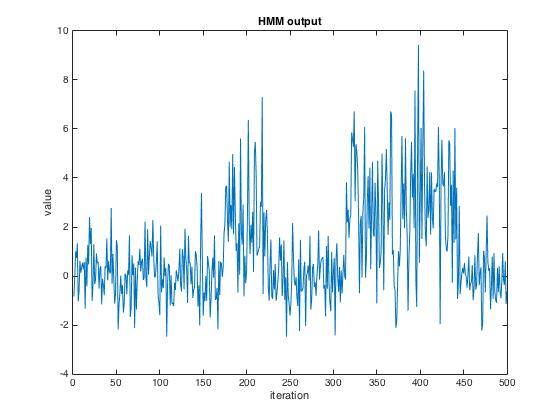
\includegraphics[width=9cm]{images/question_4_HMM_plot}
\end{figure}

We used the following code to generate this:

\begin{minted}[mathescape, linenos, numbersep=5pt, frame=lines, framesep=2mm, tabsize=4, numberblanklines=true, breaklines=true]{matlab}
%Generate random numbers from "randomly" chosen distributions
mc=MarkovChain([0.75;0.25], [0.99 0.01;0.03 0.97]);
g1=GaussD('Mean',0,'StDev',1); %distr for state 1
g2=GaussD('Mean',3,'StDev',2); %distr for state 2
h=HMM(mc, [g1; g2]);
x=rand(h, num);
%Get statistics about the numbers
disp(['mean:     ', num2str(mean(x))]);
disp(['variance: ', num2str(var(x))]);

% Question 4/5 -> plot output of random function
figure
plot(x)
title('HMM output')
xlabel('iteration')
ylabel('value')
\end{minted}

\section{} % Question 5
The following figures show the output of the HMM and the probabilities for state one and two to give a certain output value.

As we can see in the plot, we can still see what state the HMM is in. State one produces a signal with very little variance. When it is in state two, the variance is way higher, so the spikes are bigger. In this respect, the behaviour is much like the previous HMM.

Unlike the previous HMM, the mean values for both states are now the same. This makes it a bit more difficult to distinguish, since the expected values of both states are the same. As such, if we look at a single output value, we are way more likely to make a mistake when "guessing" which state produced it.

The probability distribution illustrates this statement: values close to 0 are likely to be produced by state 1, values further away are more likely to be produced by state 2.
\begin{figure}[H]
\centering
\begin{minipage}{.5\textwidth}
	\centering
	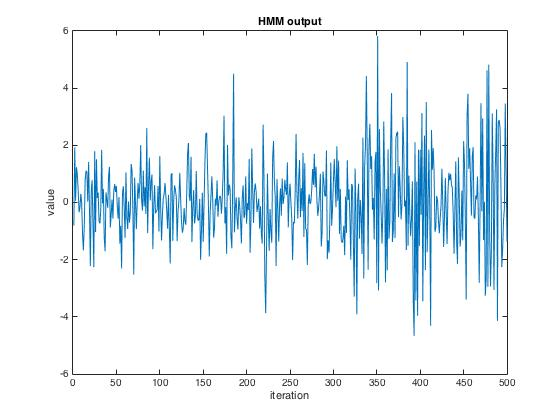
\includegraphics[width=.9\linewidth]{images/question_5_HMM_plot}
	\captionof{figure}{HMM output plot}
	\label{fig:question_5_HMM_plot}
\end{minipage}%
\begin{minipage}{.5\textwidth}
	\centering
	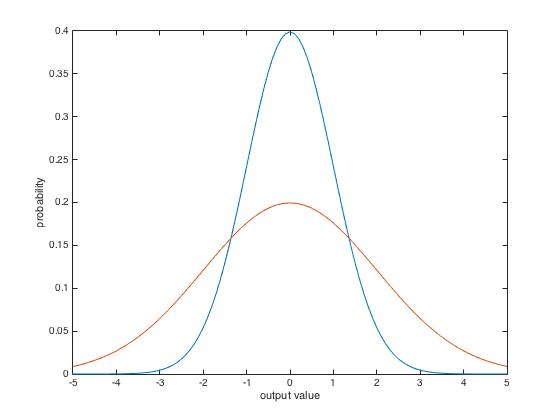
\includegraphics[width=.9\linewidth]{images/question_5_probability_distributions}
	\captionof{figure}{Probability distributions for both states}
	\label{fig:question_5_probability_distributions}
\end{minipage}
\end{figure}

\section{} % Question 6
For testing finite HMM, we introduced a special exit state. Hence, as soon as the exit state is reached no observable output is generated and the process stops. Since there are 2 states in our test case, we added a third exit state with a transition probability of $0.03$ and $0.01$. Hence, if the state $S_{t+1} = 3$, the process stops.

Observation: the lengths of some of the sequences we obtained are $200, 90, 52, 98, 66, 38, 188$...

These lengths are reasonable because the chance of getting the exit state for $S_t$ is very low ($0.03$ from State 1 to State 3 and $0.01$ from State 2 to State 3).

\section{} % Question 7
We used 2 multi-variate Gaussian distributions for generating Gaussian vector distributions as output.
Input :
g1=GaussD('Mean',[0 1],'Covariance',[2 1;1 4]); - for state 1 g2=GaussD('Mean',[3 9],'Covariance',[1 4;4 1]); - for state 2

\begin{figure}[H]
	\caption{Filling a group}
	\label{fig:question_4_HMM_plot}
	\centering
	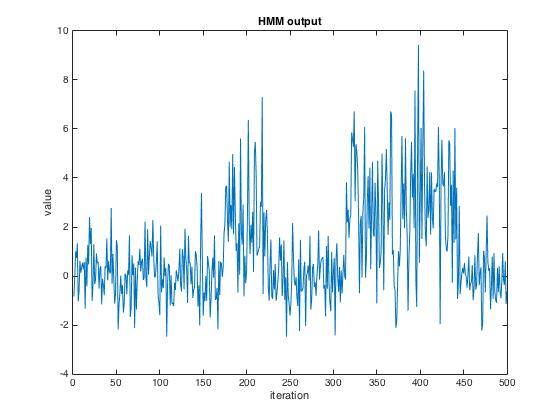
\includegraphics[width=9cm]{images/question_4_HMM_plot}
\end{figure}